\documentclass{beamer}
\usetheme{Berkeley}
\usecolortheme{seagull}
\usefonttheme{serif}
%\usefonttheme{structuresmallcapsserif} %forse un po' troppo pretenzioso

\usepackage[english,italian]{babel}
\usepackage{lipsum}
\usepackage{siunitx}
\usepackage{tikz}
\usepackage{pgfplots}
\usepackage{pgfplotstable}
\pgfplotsset{
	compat=newest,
	every tick label/.append style={font=\scriptsize},
	every node near coord/.append style={font=\scriptsize}
}
\usepgfplotslibrary{ternary}
\usetikzlibrary{calc}
\usepackage{todonotes}
\usepackage{url}
\usepackage[export]{adjustbox}
\usepackage[font={footnotesize,color=darkgray},justification=centering]{caption}

\title{OpenLDAT}
\subtitle{Un sistema di misurazione di metriche di latenza dei display}
\author{Federico Dossena}
\institute{Università degli Studi di Milano}
\date{2021-??-??}

\begin{document}
	
\begin{frame}
	\titlepage
\end{frame}

\section{Introduzione}
\begin{frame}
	\frametitle{Introduzione}
	\begin{itemize}
		\item Progetto nato dall'esigenza di \textcolor{blue}{misurare la latenza totale di un sistema} in modo automatico
		\item \textcolor{blue}{Nessun dispositivo simile sul mercato}, solitamente si usa un mouse con collegato un LED e una telecamera ad alta velocità
		\item \textcolor{blue}{OpenLDAT può misurarla in modo automatico}, e può fare anche molto altro
		\item Progetto totalmente \textcolor{blue}{libero}
	\end{itemize}
	\begin{block}{Latenza totale del sistema}
		Tempo che intercorre tra un'azione nel mondo fisico, come un click del mouse, e la visualizzazione del risultato sul display.
	\end{block}
\end{frame}
\begin{frame}[shrink=10]
	\frametitle{Nvidia LDAT}
	\begin{columns}
		\column{0.5\textwidth}
		\begin{itemize}
			\item A Settembre 2020, Nvidia ha inviato dei prototipi di \textcolor{blue}{Nvidia LDAT} ad alcuni giornalisti specializzati, ma poi \textcolor{blue}{non ha commercializzato il prodotto}
			\item Il dispositivo permetteva di misurare la \textcolor{blue}{latenza totale del sistema} in modo manuale o semi-automatico
			\item Il progetto \textcolor{blue}{OpenLDAT} vuole ricreare questo dispositivo, aggiungere più funzioni, e utilizzarlo per testare dei display
		\end{itemize}
		\column{0.5\textwidth}
		\begin{figure}
			\centering
			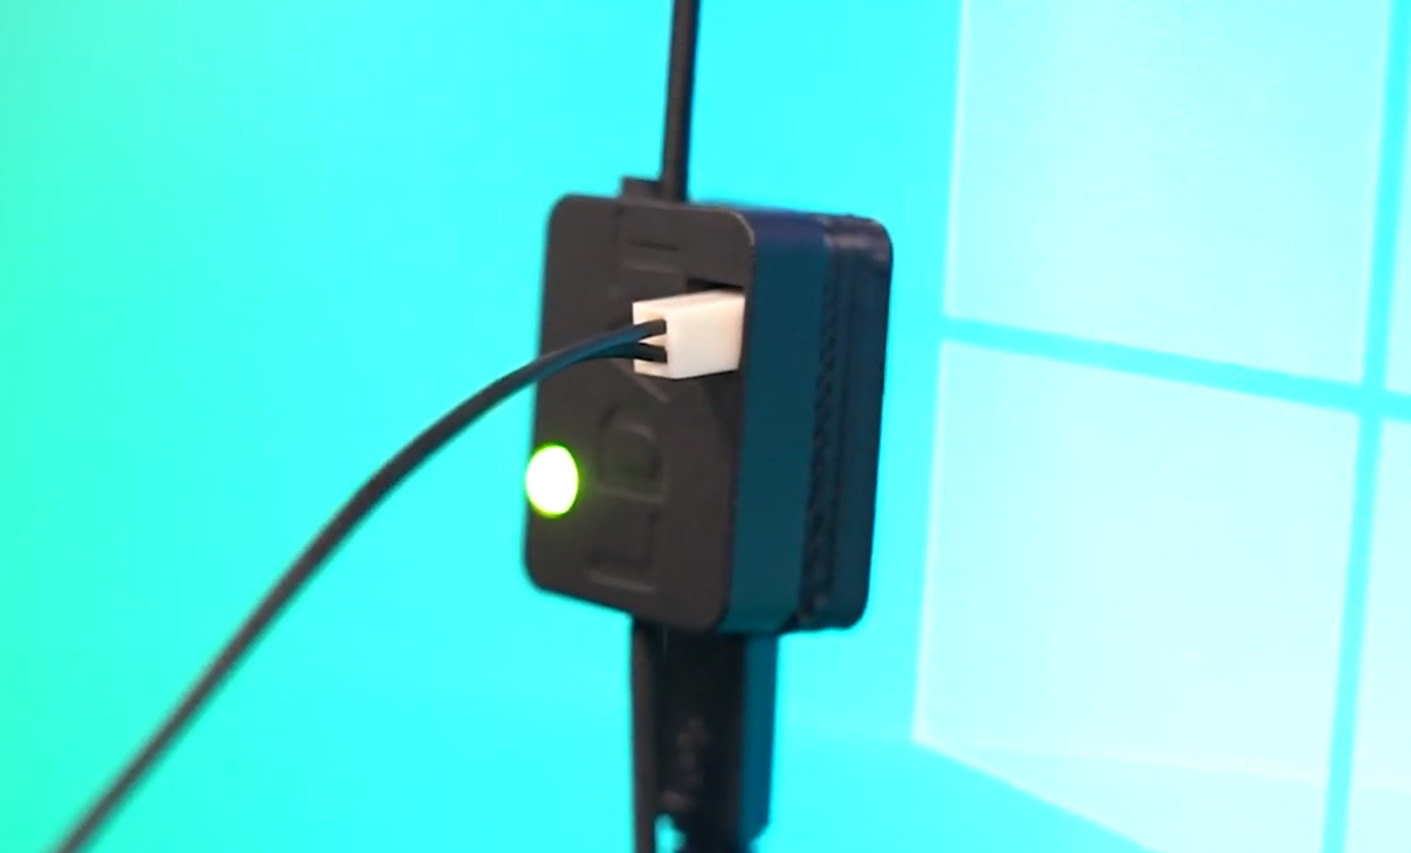
\includegraphics[width=\textwidth]{StatoDellArte_files/nvldat_front.jpg}
			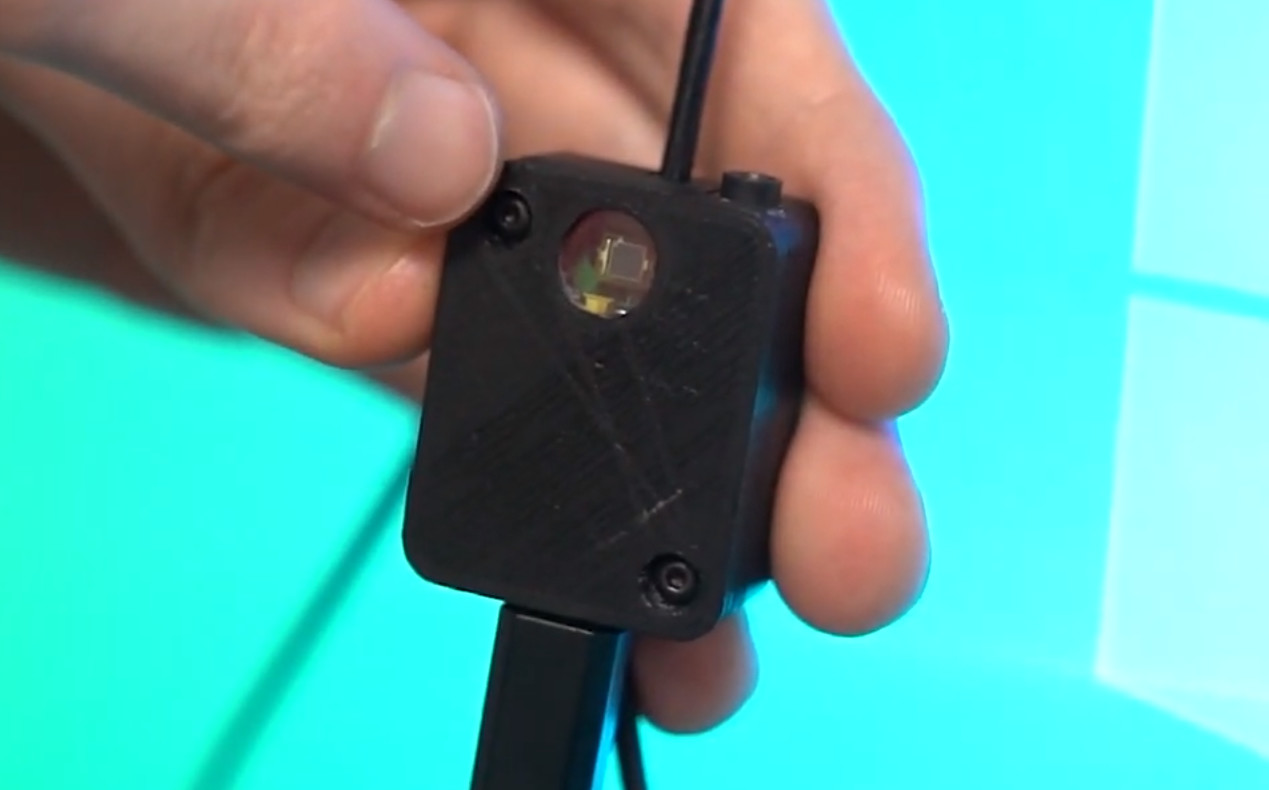
\includegraphics[width=\textwidth]{StatoDellArte_files/nvldat_back.jpg}
			\caption*{Dispositivo Nvidia LDAT}
		\end{figure}
		
	\end{columns}
	
\end{frame}

\section{Dispositivo}
\begin{frame}[shrink=10]
	\frametitle{Dispositivo OpenLDAT (1)}
	\begin{columns}
		\column{0.5\textwidth}
		\begin{itemize}
			\item Microcontroller \textcolor{blue}{ATmega32U4}
			\item Fototransistor \textcolor{blue}{ALS-PT19} con \textcolor{blue}{4 livelli di gain} del sensore controllabili via software
		\end{itemize}
		\column{0.5\textwidth}
		\begin{itemize}
			\item \textcolor{blue}{PCB} personalizzato
			\item Campionamento fino a \textcolor{blue}{\textasciitilde 30kHz 10-bit}
			\item Comunicazione via USB HID e CDC Serial, \textcolor{blue}{nessun driver richiesto}
		\end{itemize}
	\end{columns}
	\begin{figure}
		\centering
		\adjincludegraphics[trim={{.10\width} 0 {.20\width} 0},clip,height=0.55\textheight]{Dispositivo_files/assembly_10.jpg}
		\adjincludegraphics[trim={{.12\width} 0 {.18\width} 0},clip,height=0.55\textheight]{Dispositivo_files/assembly_09.jpg}
		\caption*{Hardware del dispositivo OpenLDAT}
	\end{figure}
\end{frame}
\begin{frame}
	\frametitle{Dispositivo OpenLDAT (2)}
	\begin{columns}
		\column{0.5\textwidth}
		\begin{itemize}
			\item Generazione dei \textcolor{blue}{click automatica o manuale} tramite input esterno
			\item \textcolor{blue}{LED per validazione} con telecamera ad alta velocità
			\item \textcolor{blue}{Case stampabile} in 3D
			\item \textcolor{blue}{Poco costoso e facile da realizzare} anche da un maker
		\end{itemize}
		\column{0.5\textwidth}
		\begin{figure}
			\adjincludegraphics[trim={{.22\width} 0 {.22\width} 0},clip,width=\textwidth]{Dispositivo_files/assembly_15.jpg}
			\caption*{Dispositivo OpenLDAT assemblato}
		\end{figure}
	\end{columns}
\end{frame}

\section{Applicazione}
\begin{frame}[shrink=15]
	\frametitle{Applicazione OpenLDAT (1)}
	\begin{columns}
		\column{0.5\textwidth}
		\begin{itemize}
			\item \textcolor{blue}{Applicazione grafica} Java SE e OpenGL
			\item Permette di \textcolor{blue}{configurare, eseguire i test, e visualizzarne i risultati} in modo semplice
		\end{itemize}
		\column{0.5\textwidth}
		\begin{itemize}
			\item \textcolor{blue}{Esportazione dei dati} per un analisi esterna
			\item \textcolor{blue}{Include un manuale} che spiega i test
			\item \textcolor{blue}{Multipiattaforma} (Windows, GNU/Linux, MacOS)
		\end{itemize}
	\end{columns}
	\begin{figure}
		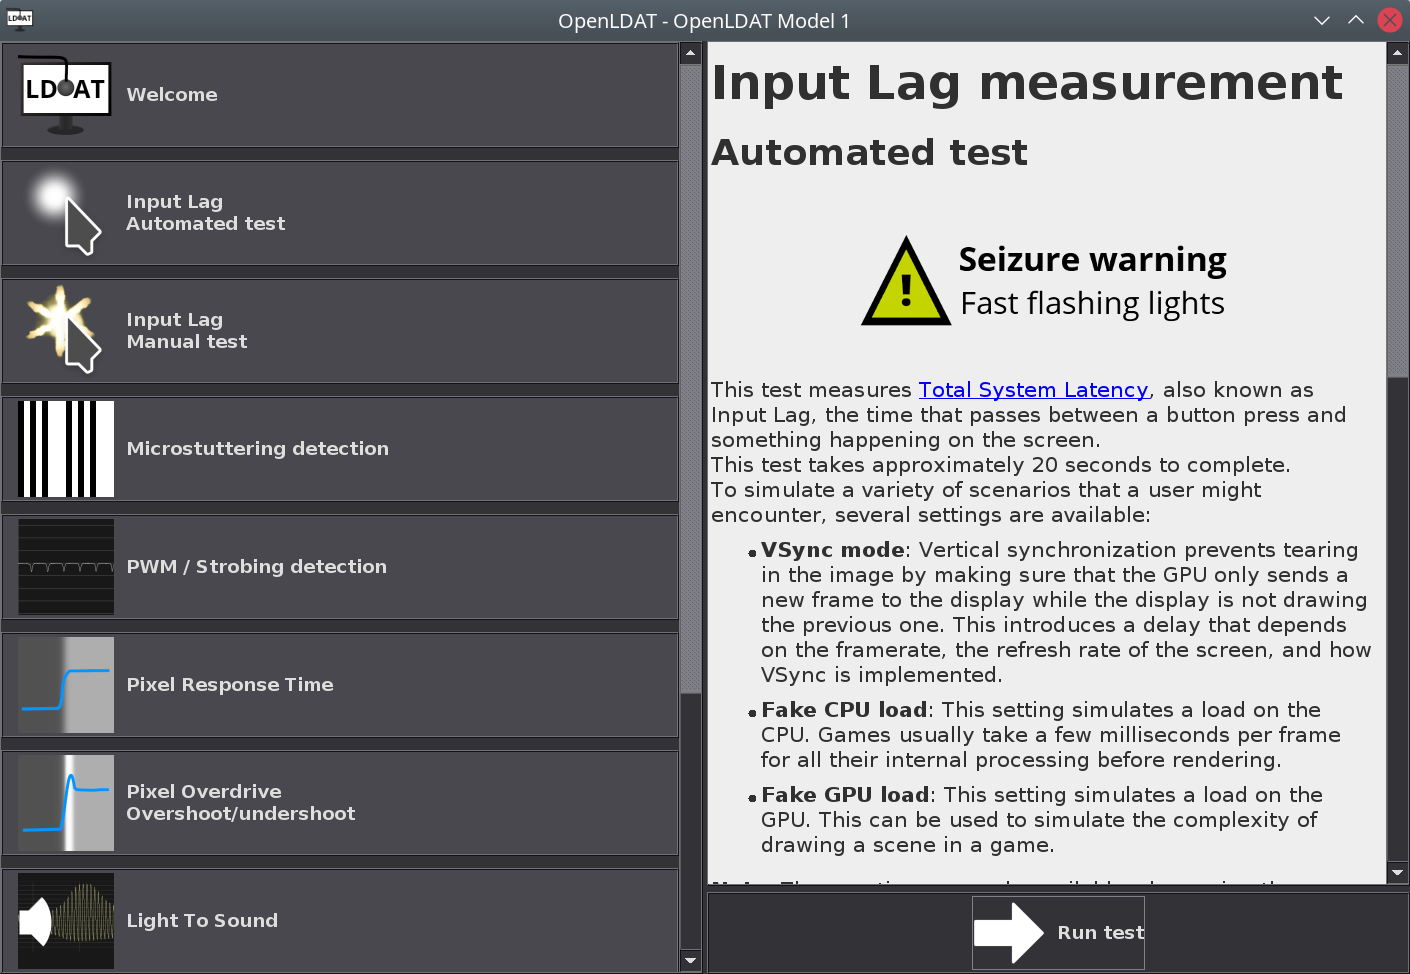
\includegraphics[height=0.7\textheight]{Applicazione_files/gui_mainMenu2.png}
		\caption*{Schermata principale dell'applicazione}
	\end{figure}
\end{frame}
\begin{frame}[shrink=7]
	\frametitle{Applicazione OpenLDAT (2)}
	Elenco dei test:\begin{itemize}
		\item \textcolor{blue}{Latenza totale del sistema}:\begin{itemize}
			\item \textcolor{blue}{Test automatico} con OpenGL e generazione automatica dei click
			\item \textcolor{blue}{Test manuale} utilizzando un'applicazione e la generazione automatica dei click o un mouse/controller modificato
		\end{itemize}
		\item \textcolor{blue}{Rilevamento del microstuttering}: rileva perdita/duplicazione di fotogrammi
		\item \textcolor{blue}{Rilevamento di PWM e noise}: rileva la frequenza del lampeggio della retroilluminazione e altri tipi di noise
		\item \textcolor{blue}{Tempi di risposta dei pixel}: misura il tempo di transizione dei pixel
		\item \textcolor{blue}{Misurazione dell'overdrive}: misura l'errore commesso durante la transizione dei pixel
		\item \textcolor{blue}{Light To Sound}: permette di ascoltare il segnale dal sensore, utile per rilevare fonti di rumore, ma anche per divertimento
	\end{itemize}
\end{frame}
\begin{frame}
	\frametitle{Applicazione OpenLDAT (3)}
	\begin{figure}
		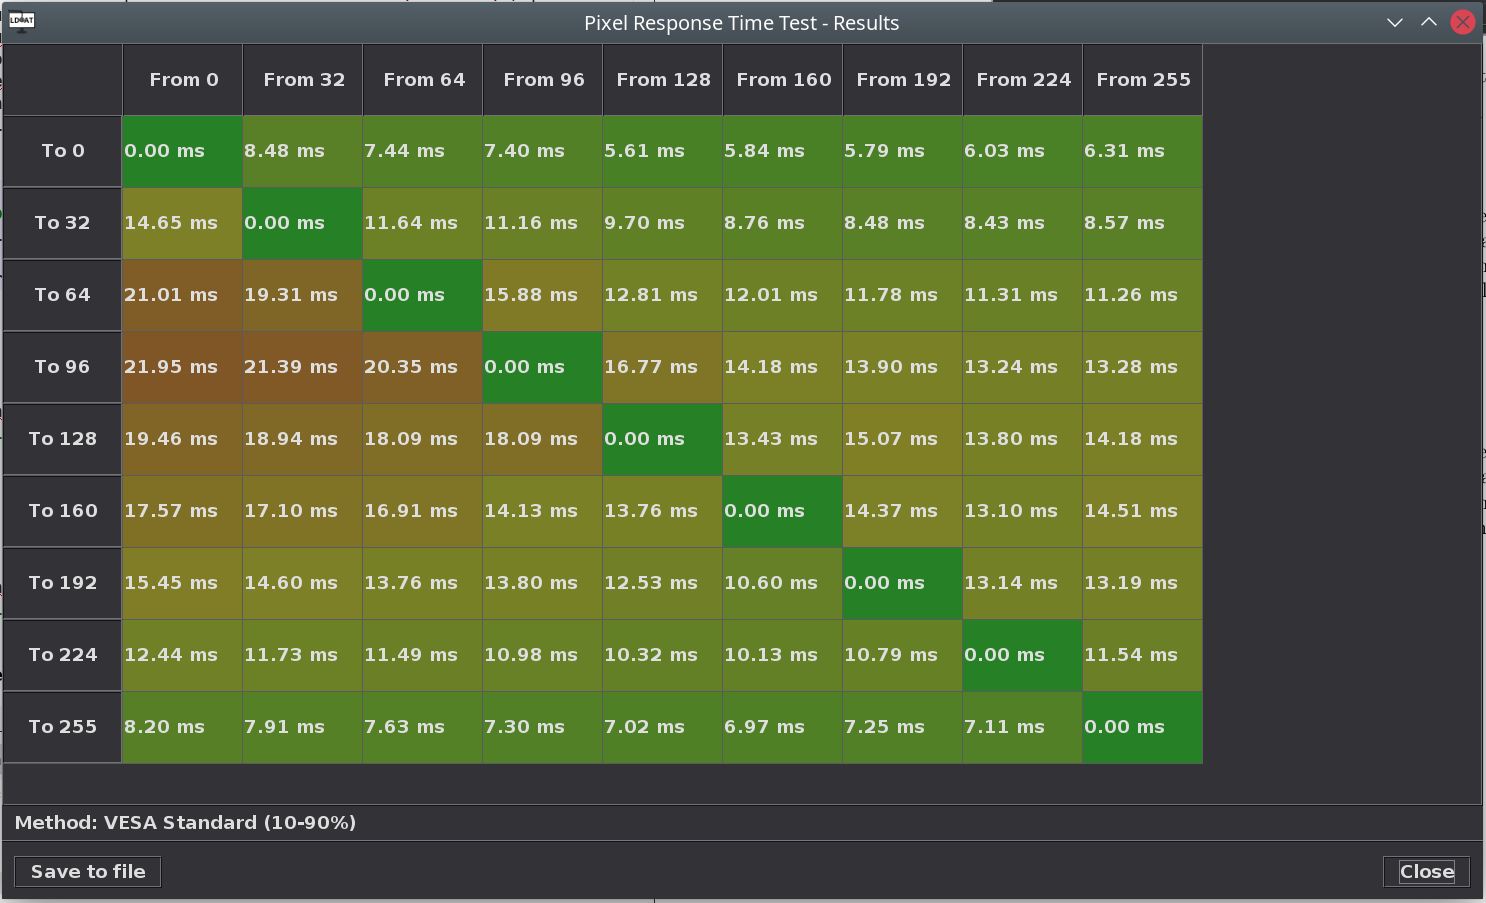
\includegraphics[width=\textwidth]{Applicazione_files/gui_pixelresponse_results.png}
		\caption*{Esempio di risultati di un test dei tempi di risposta dei pixel (AOC Q2770P)}
	\end{figure}
	
\end{frame}

\section{Risultati sperimentali}
\begin{frame}
	\frametitle{Input lag (1)}
	\lipsum[1]
\end{frame}
\begin{frame}
	\frametitle{Input lag (2)}
	\lipsum[1]
\end{frame}
\begin{frame}
	\frametitle{PWM e noise}
	\lipsum[1]
\end{frame}
\begin{frame}
	\frametitle{Risposta dei pixel}
	\lipsum[1]
\end{frame}
\begin{frame}
	\frametitle{Overdrive}
	\lipsum[1]
\end{frame}
\begin{frame}
	\frametitle{Microstuttering}
	\lipsum[1]
\end{frame}

\section{Conclusioni}
\begin{frame}
	\frametitle{Conclusioni}
	\lipsum[1]
\end{frame}
\begin{frame}
	\frametitle{Grazie per l'attenzione}
	\centering
	Per maggiori informazioni:
	\textcolor{blue}{\url{https://openldat.fdossena.com}}
\end{frame}

\end{document}
